\documentclass{article}


% if you need to pass options to natbib, use, e.g.:
%     \PassOptionsToPackage{numbers, compress}{natbib}
% before loading neurips_2022


% ready for submission
\usepackage[final]{neurips_2022}
% \usepackage[nonatbib]{neurips_2022}


% to compile a preprint version, e.g., for submission to arXiv, add add the
% [preprint] option:
%     \usepackage[preprint]{neurips_2022}


% to compile a camera-ready version, add the [final] option, e.g.:
%     \usepackage[final]{neurips_2022}


% to avoid loading the natbib package, add option nonatbib:
%    \usepackage[nonatbib]{neurips_2022}


\usepackage[utf8]{inputenc} % allow utf-8 input
\usepackage[T1]{fontenc}    % use 8-bit T1 fonts
\usepackage{hyperref}       % hyperlinks
\usepackage{url}            % simple URL typesetting
\usepackage{booktabs}       % professional-quality tables
\usepackage{amsfonts}       % blackboard math symbols
\usepackage{nicefrac}       % compact symbols for 1/2, etc.
\usepackage{microtype}      % microtypography
\usepackage{xcolor}         % colors
\usepackage{enumitem}       % enumerate

\usepackage{listings}       % code
\usepackage{graphicx} %插入图片的宏包
\usepackage{float} %设置图片浮动位置的宏包
\usepackage{subfigure} %插入多图时用子图显示的宏包
\usepackage{amsmath}



\title{Exploring the Efficacy of BERT \\ on a Fine-Grained Emotion Dataset : GoEmotions}


% set vertical space between authors' names and addresses
\author{
  \vspace{0.2cm}
  Liangshen Yin \\
  \vspace{0.2cm}
  Shanghai Jiao Tong University \\
  \texttt{hnyls2002@sjtu.edu.cn}
}


\begin{document}

\maketitle

\begin{abstract}
  In this paper, We focus on a fine-grained emotions classification dataset : GoEmotions, published by Google Research. The GoEmotions dataset is not so popular, and there are few public results for comparison. We explore the efficacy of BERT, a pre-trained language model, on this dataset.
  Our work is mainly fine-tuning on a BERT-base model, and we have tried many different hyperparameters and fine-tuning strategies. However, the performance of our model is still far below the state-of-the-art result.
\end{abstract}

\section{Introduction}
Fine-grained emotion classification is a challenging task in natural language processing as it requires the model to discern subtle differences between emotions. The GoEmotions dataset \cite{goemotions} contains 58k curated Reddit comments labeled with 27 emotion categories and Neutral, making it an ideal benchmark for evaluation. In this paper, we explore the efficacy of BERT, a pre-trained language model \cite{bert}, on this dataset. The code for our experiments is available at \url{https://github.com/hnyls2002/KFC-emo}.

Given our resource constraints, we adopt a bunch of strategies of fine-tuning the BERT model provided by \texttt{HuggingFace} on the GoEmotions dataset, rather than undertaking the daunting task of pre-training on a massive corpus. The pre-trained BERT model we used is \texttt{bert-base-uncased}, which has 12 layers, 768 hidden size, 12 attention heads, and 110M parameters.

Our model is simple and consists of a BERT model and one or two fully connected layers. We observe that adding more layers does not necessarily improve performance but increases computation time. Additionally, we experimented with different fine-tuning approaches, such as freezing and unfreezing the BERT model, expanding the dataset and so on. The current best performance we achieved is a macro-F1 score of 0.39 on the test set, which is far below the baseline (also a state-of-the-art result) of 0.46.

Additionally, apart from fine-grained emotion classification in the GoEmotions dataset, we also experimented with two other classification tasks: sentiment grouping and Ekman's taxonomy. The sentiment classification task comprises three classes: \texttt{positive, negative, and ambiguous}. On the other hand, Ekman's taxonomy categorizes emotions into six classes: \texttt{anger, disgust, fear, joy, sadness, and surprise}.

\newpage
\section{Related Work}

\subsection{BERT model}

Pre-trained language models have recently gained dominance in many NLP tasks, including Question Answering, Natural Language Inference, and Sentiment Analysis. However, in the field of fine-grained emotion classification, the efficacy of pre-trained language models seems to be limited.

Among the pre-trained language models, BERT \cite{bert} is the most widely used. It is a multi-layer bidirectional Transformer encoder designed for masked language modeling objectives. The base model comprises approximately 110M parameters while the large model consists of 340M parameters, necessitating enormous amounts of unlabeled data for pretraining. Following the emergence of BERT, various other pre-trained models have been developed to improve its performance or mitigate training time, such as RoBERTa \cite{roberta}, ALBERT \cite{albert}, and so on.

\subsection{Baseline for GoEmotions}

In the paper \cite{goemotions} detailing the GoEmotions dataset, Google Research authors proposed a baseline model based on BERT. They achieved a macro F1 score of 0.46 on the test set, which is currently the state-of-the-art performance for this dataset. However, with no additional public results available, it is unclear how effective this baseline is.

The baseline model proposed by Google Research is as simple as ours. It just adds one dense output layer on top of the BERT model, keeping most of the hyperparameters unchanged, only modifying the batch size to 16. Moreover, they also provided an additional baseline model, which is a bidirectional LSTM and its performance is not so good.

As the GoEmotions dataset has minimal popularity and does not attract significant attention or participation, there are no other publicly available results for comparison. Therefore, we cannot compare our results with other models.

\section{Task}

\subsection{Features of Dataset}

The GoEmotions dataset is collected from Reddit comments, so it contains a lot of informal language and slang, which makes it challenging to classify. And the text classified to be \texttt{neutral} comprises a large proportion of the dataset, up to $26.5\%$. The following figure shows the distribution of each emotion in the GoEmotions dataset (the \texttt{neutral} class is not included).

\begin{figure}[H]
  \centering
  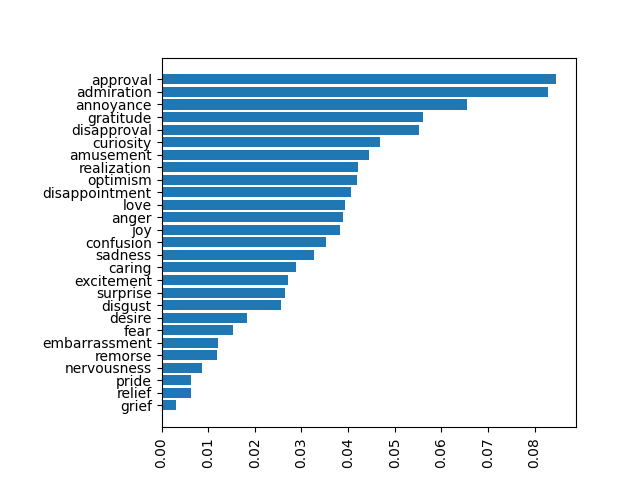
\includegraphics[width=0.8\textwidth]{img2.png}
  \caption{Emotions's distribution}
  \label{fig1:label}
\end{figure}

It is worth noting that the text in the GoEmotions dataset can be labeled with multiple emotions. So the classification task is a multi-label classification task, not a multi-class classification task. The following figure shows a few examples of the GoEmotions dataset.

\begin{table}[H]
  \centering
  \renewcommand\arraystretch{1.5}
  \begin{tabular}{p{0.6\textwidth}p{0.2\textwidth}}
    \hline
    \textbf{Sample Text}                                                                                                                       & \textbf{Label(s)}                          \\
    \hline
    \hline
    Just thinking about all the stupid stuff I did  as a kid makes me very afraid for my 5 year old.                                           & \texttt{fear}                              \\
    \hline
    Wow! You must have pretty low standards for teachers in your state/school! I guess that's why Massachusetts is always first for education. & \texttt{admiration, curiosity, nervouness} \\
    \hline
    I think someone else should open a drive through so I can enjoy the flavours without the dishes aha                                        & \texttt{joy}                               \\
    \hline
    Lol you're an idiot.                                                                                                                       & \texttt{amusement}                         \\
    \hline
    Agree. Not a perfect coach but pretty, pretty good                                                                                         & \texttt{admiration}                        \\
    \hline
  \end{tabular}
  \vspace{0.2cm}
  \caption{Examples of GoEmotions dataset}
\end{table}

\section{Approach}

\subsection{Model}

Our model is simply a BERT model with one or two fully connected layers. The BERT model is used to extract features from the text, and the fully connected layer is used to classify the emotion. The following figure shows the structure of our model.

\begin{figure}[H]
  \centering
  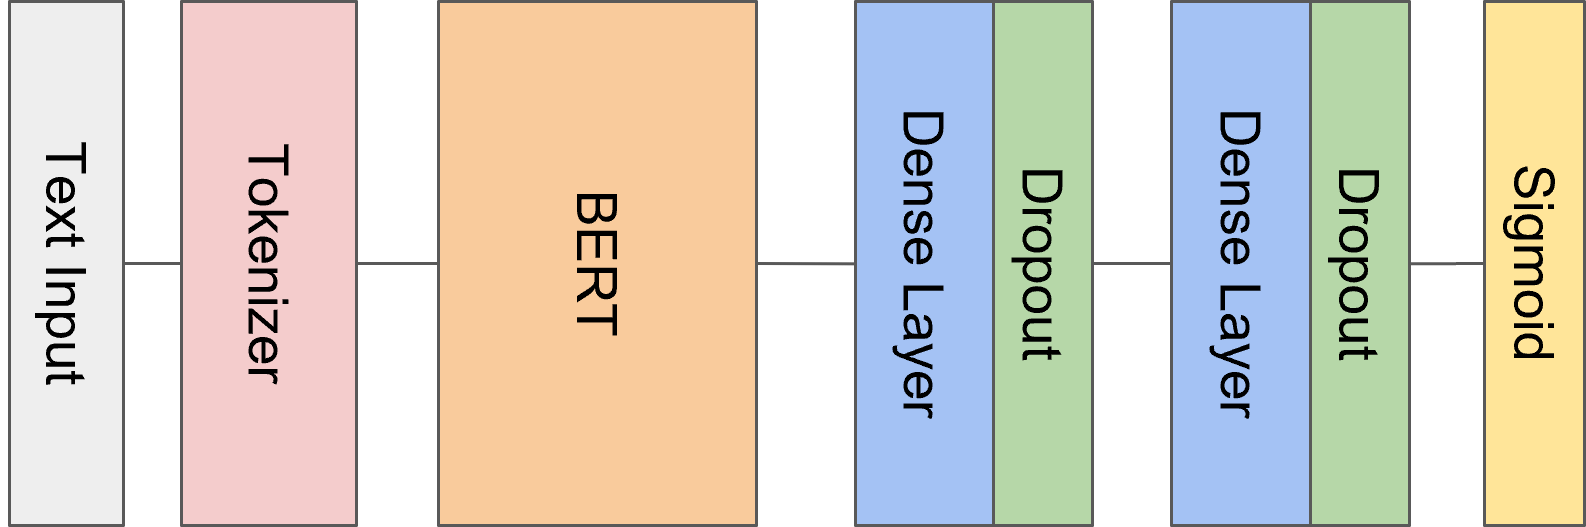
\includegraphics[width=0.8\textwidth]{img3.png}
  \caption{Model structure}
\end{figure}

\subsubsection{Tokenization and BERT Model}

The tokenizer and BERT model are both imported from the \texttt{HuggingFace.transformers} library. The text input is first tokenized by the tokenizer, and then the tokenized text is fed into the BERT model. All the hyperparameters of the BERT model are kept unchanged, and the output of the BERT model is the last hidden state of the \texttt{[CLS]} token.

\subsubsection{Inference Layers}

In the above figure, our model contains two fully connected layers to do the Inference. However, in the following experiments, we find that adding more layers does not necessarily improve performance but increases computation time. Basically, they are almost the same in performance. So in the next sections of the paper, we would not mainly discuss the number of layers in the inference layers.

\subsubsection{Loss Function}

As mentioned above, the GoEmotions dataset is a multi-label classification task. So we use the \texttt{BCEWithLogitsLoss} loss function provided by \texttt{PyTorch} to calculate the loss. Suppose the direct output of the last layer is the digit of each emotion, then the loss function is defined as follows:

$$
  \text{Loss} =  \frac{1}{N}\sum_{i = 1} ^{N} \left(y_i \log (\sigma(x_i)) + (1 - y_i)\log(1 - \sigma(x_i))\right)
$$

\subsubsection{Settings of Hyperparameters}

The settings of hyperparameters in the SOTA model are not fully given in the paper \cite{goemotions}, so we have to try different hyperparameters to find the best one.

The batch size is set to 16, larger batch size would cause obviously overfitting. The learning rate is fixed as 5e-5 in the SOTA model, but we use a dynamic learning rate, which is adjusted by the \texttt{lr\_scheduler.CyclickLR("triangular")}, from 1e-5 to 5e-5.

We do not change the hidden layer dropout probability in the BERT model. In some of our experiments, for the last Inference layers, we set the dropout probability to 0.1 or 0.2, and the performance is slightly improved.

In most of our experiments, the epochs for training are set to 2 or 3, because the models will probably overfit after 3 epochs. However, the total epochs in the fine-tuning process with freezing BERT model are slightly different, as it have two different stages, which will be introduced later.

\subsection{Optimization for threshold}

28 kinds of emotions have different distributions in the dataset, as shown in Figure\ref{fig1:label}. And the loss function is just an average of all kinds, so when we decrease the loss, different kinds of emotions have different rates of decrease. Therefore, we need to set different thresholds for different emotions to get the best results.

Here we choose the macro F1 score as the evaluation metric. To maximize the macro F1 score, we try to maximize the F1 score of each emotion first. For each epoch after we have trained the model through the training set, we set the best threshold according the performance on the training set, hoping that this threshold can also perform well on the validation set. The following figure shows the F1 score and threshold of each emotion in some experiment.

\begin{figure}[H]
  \centering
  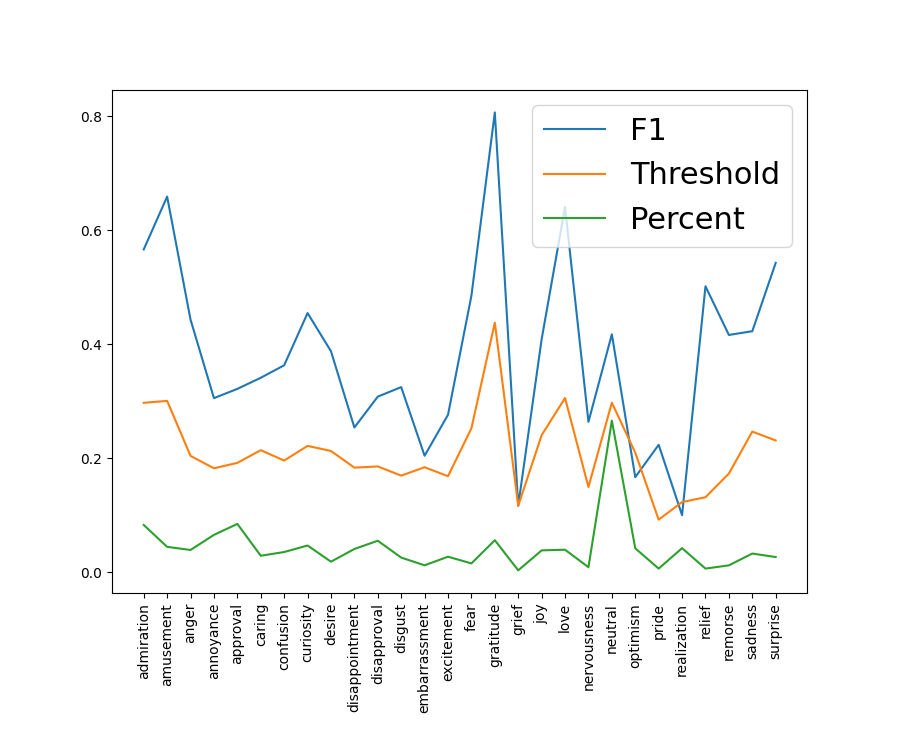
\includegraphics[width=0.8\textwidth]{img4.png}
  \caption{F1 score and threshold of each emotion}
\end{figure}

We can notice that the F1 score curve and threshold curve are very similar. The emotions with higher F1 scores are also the emotions with higher thresholds.
Although the F1 score is actually "chosen by the threshold", the F1 score is still the best we can achieve after training some epochs.

The similarity of the two curves also demonstrates that, when our model has better performance on some emotion, then the output \texttt{logits} of this emotion will be easier to classify, that is why the threshold of this emotion is higher.

We can also notice that some emotions have very low F1 scores, such as \texttt{grief, pride}, while \texttt{gratitute, love, admiration} have very high F1 scores.
Looking at the distribution curve, it is not difficult to find that the \texttt{grief, pride} are very rare in the dataset, while the \texttt{gratitute, love, admiration} are more common. The insufficient data of some emotions may be one of the reasons for the poor performance on GoEmotions dataset.

\subsection{Freezing BERT Model and Two-Stage Fine-Tuning}

Two stage fine-tuning is a common strategy in the fine-tuning process of BERT model. That is because the billions of parameters in the BERT model are well trained on a large corpus, if we repeatedly train the BERT model on a small dataset, it will cause overfitting. So we apply the two-stage fine-tuning strategy to avoid overfitting.

\begin{figure}[H]
  \centering
  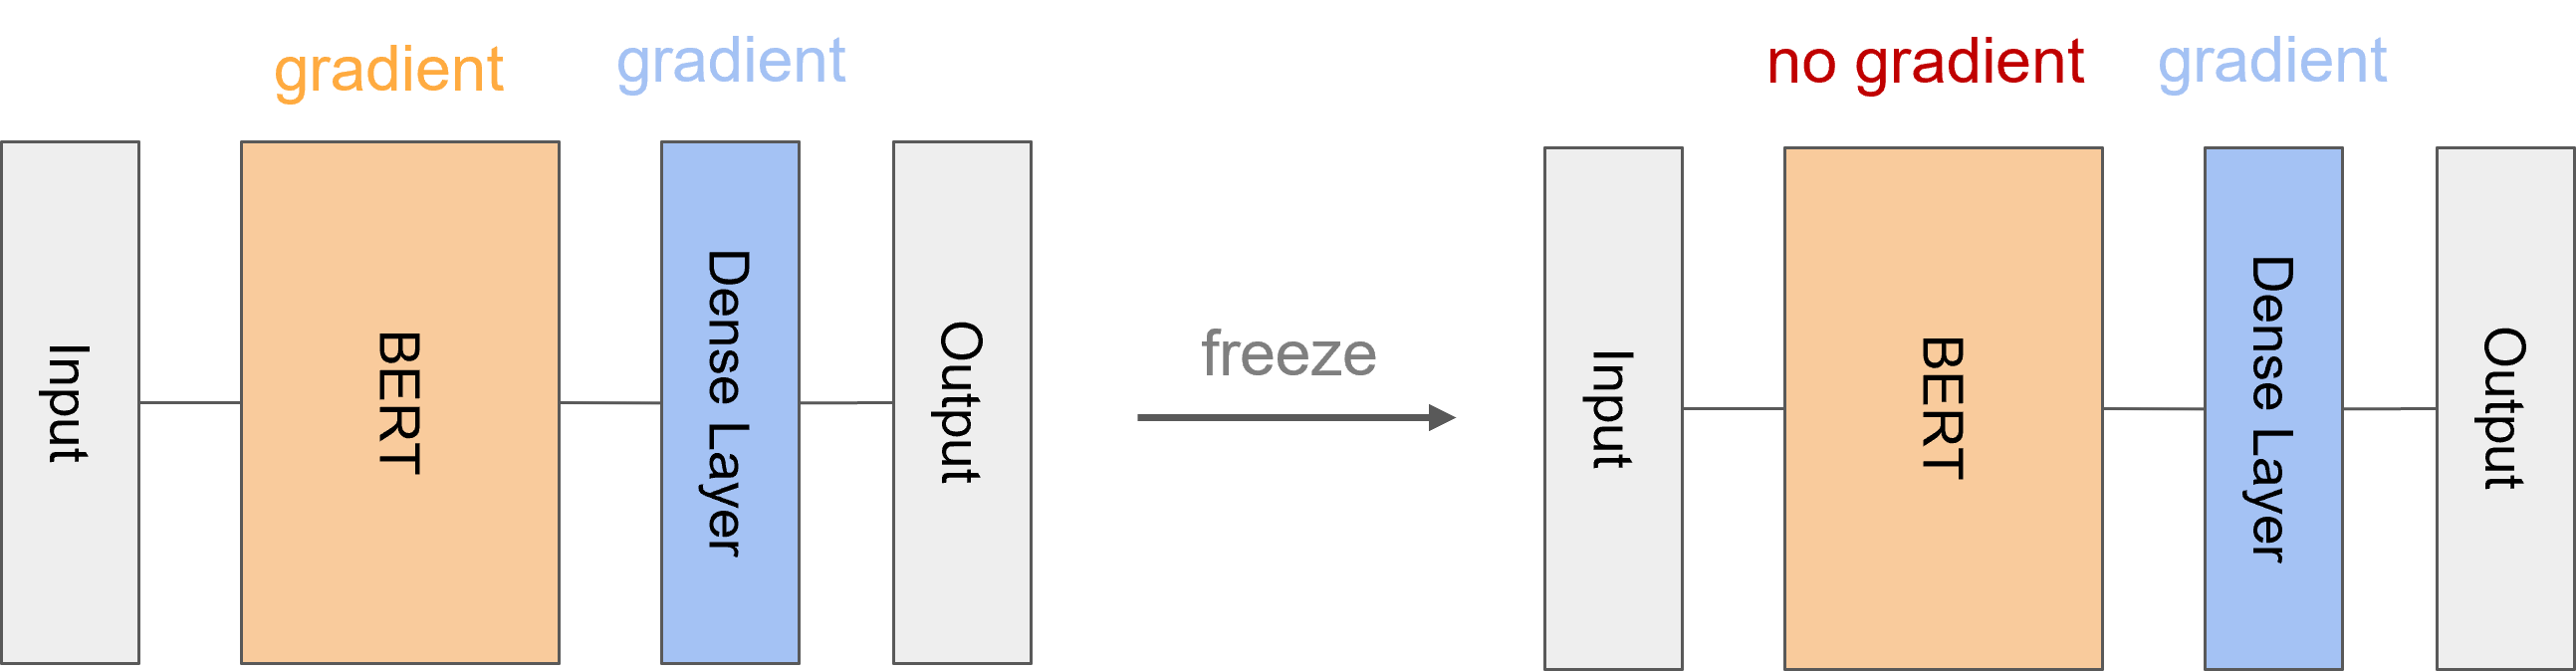
\includegraphics[width=0.8\textwidth]{img5.png}
  \caption{Two-stage fine-tuning}
\end{figure}


\begin{enumerate}[label=(\alph*)]
  \item The first stage is to train our model without freezing the parameters inside BERT, this lasts two or three epochs.
  \item In the second stage, we reset all the parameters in our inference layers, and freeze all the parameters in BERT model, then retrain the model for two or three epochs.
\end{enumerate}

\subsection{Expanding the Dataset}

The GoEmotions dataset is not large enough, so we try to expand the dataset by concatenating two text in the dataset, and also merge their labels. For example, if we have two texts with labels \texttt{[joy, admiration]} and \texttt{[joy, amusement]}, then we can get a new text with label \texttt{[joy, admiration, amusement]}.

However, this simple method would cause some problems, as the emotions are not orthogonal. When we concatenate two sentences with opposite emotions, the new sentence may be meaningless. For example, \texttt{I love you} plus \texttt{I hate you} would be \texttt{I love you.I hate you}, which is so weird.

Although this method seems to have some problems, we still try it in our experiments. We concatenate two texts randomly, expand the training set to 1 million texts. However, the training time is too long, we only train the model for one epoch without freezing BERT model. After that, we continue to train the model for another several epochs, but this time we freeze the BERT model. The performance is not improved significantly, but not so bad.

\section{Experiments}

This section presents the results of our experiments. As previously mentioned, we experimented with various hyperparameters and fine-tuning strategies. Our evaluation metric is the macro F1 score, along with the weighted F1 score and accuracy for reference. It should be noted that accuracy is not an ideal metric for multi-label classification tasks because all dimensions of the prediction must be correct for a text to be accurately labeled.

The following table shows the results of all our experiments.

\begin{table}[H]
  \centering
  \renewcommand\arraystretch{1.5}
  \begin{tabular}{p{0.5\textwidth}p{0.1\textwidth}p{0.1\textwidth}p{0.1\textwidth}p{0.1\textwidth}}
    \hline
    \textbf{Experiment}                                                                                                          & \textbf{Epochs} & \textbf{M-F1} & \textbf{W-F1} & \textbf{Acc} \\
    \hline
    \hline
    \textbf{DenseLayer(1)} + \textbf{Dynamic lr}                                                                                 & 2               & 0.27          & N/A           & 0.22         \\
    \hline
    \textbf{DenseLayer(1)} + \textbf{Fixed lr(5e-5)}                                                                             & 4               & 0.26          & N/A           & 0.23         \\
    \hline
    \textbf{DenseLayer(1)} + \textbf{Fixed lr(5e-5)}  + \textbf{TwoStage}                                                        & 2 + 2(frz)      & 0.29          & N/A           & 0.24         \\
    \hline
    \textbf{DenseLayer(1)} + \textbf{Dynamic lr} + \textbf{TwoStage}                                                             & 2 + 4(frz)      & 0.29          & N/A           & 0.24         \\
    \hline
    \textbf{DenseLayer(1)} + \textbf{Dynamic lr} + \textbf{Dropout(0.1)} +  \textbf{TwoStage}                                    & 2 + 6(frz)      & 0.29          & N/A           & 0.24         \\
    \hline
    \textbf{DenseLayer(1)} + \textbf{Dynamic lr} + \textbf{Dropout(0.1)} + \textbf{TwoStage} +  \textbf{OptOnThreshold}          & 2 + 3(frz)      & 0.38          & 0.44          & 0.23         \\
    \hline
    \textbf{DenseLayer(1)} + \textbf{Dynamic lr} + \textbf{Dropout(0.1)} +  \textbf{TwoStage} + \textbf{OptOnThreshold}          & 4 + 4(frz)      & 0.39          & 0.44          & 0.25         \\
    \hline
    \textbf{DenseLayer(1)} + \textbf{Fixed lr(5e-5)} + \textbf{OptOnThreshold} + \textbf{ExpanedDataset}                         & 1               & 0.35          & 0.41          & 0.18         \\
    \hline
    \textbf{DenseLayer(2)} + \textbf{Dynamic lr} + \textbf{Dropout(0.1)} + \textbf{TwoStage} + \textbf{OptOnThreshold}           & 4 + 3(frz)      & 0.39          & 0.44          & 0.23         \\
    \hline
    \textbf{DenseLayer(2)} + \textbf{Dynamic lr} + \textbf{Dropout(0.2)} + \textbf{TwoStage} + \textbf{OptOnThreshold}           & 4 + 3(frz)      & 0.39          & 0.45          & 0.24         \\
    \hline
    \textbf{DenseLayer(1)} + \textbf{Dynamic lr} + \textbf{Dropout(0.1)} + \textbf{OptOnThreshold} + \textbf{TwoStageOnExtended} & 1 + 3(frz)      & 0.37          & 0.42          & 0.24         \\
    \hline
  \end{tabular}
  \vspace{0.2cm}
  \caption{Results of all experiments}
\end{table}

\subsection{Sentimentment and Ekman}

We also experimented with two other classification tasks: sentiment grouping and Ekman's taxonomy. The mapping from emotions to sentiment and Ekman's taxonomy is shown in the following table, which achieves good results nearly reaching the SOTA result.

\begin{figure}[H]
  \centering
  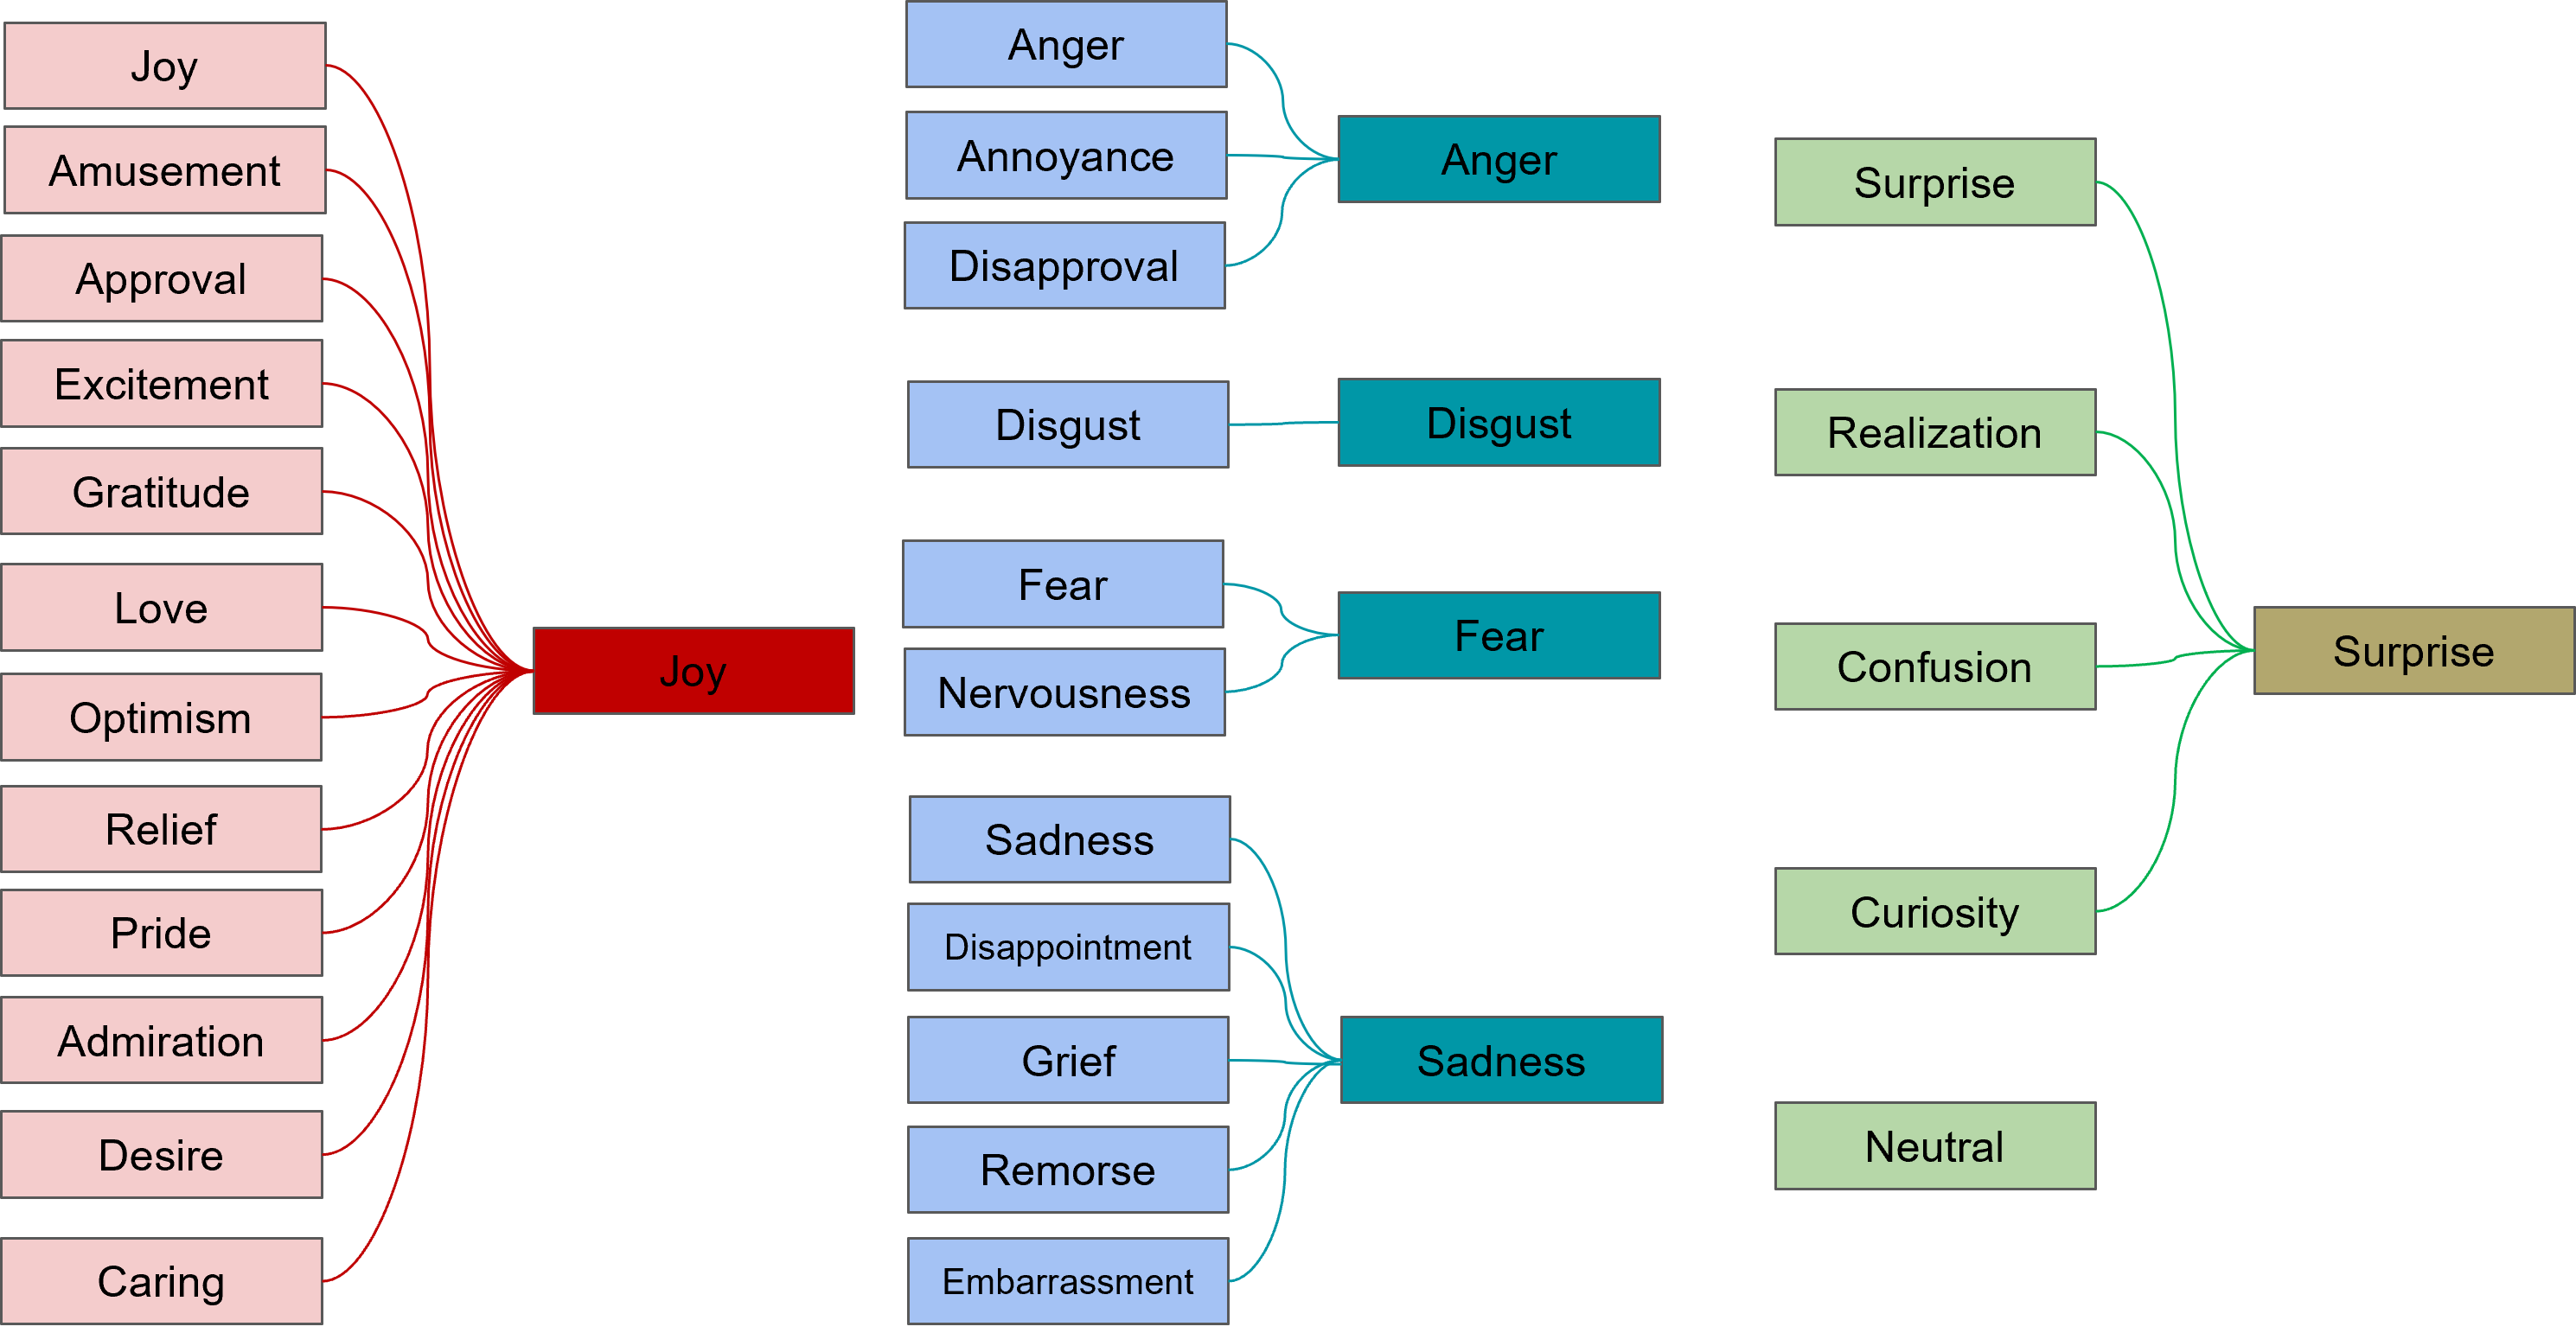
\includegraphics[width=0.8\textwidth]{img1.png}
  \caption{Mapping from emotions to sentiment and Ekman's taxonomy}
\end{figure}

And the results of our experiments are shown in the following table.

\begin{table}[H]
  \centering
  \renewcommand\arraystretch{1.5}
  \begin{tabular}{p{0.1\textwidth}p{0.35\textwidth}p{0.1\textwidth}p{0.1\textwidth}p{0.1\textwidth}p{0.1\textwidth}}
    \hline
    \textbf{Classify} & \textbf{Experiment}                                                                                                 & \textbf{Epochs} & \textbf{M-F1} & \textbf{W-F1} & \textbf{Acc} \\
    \hline
    \hline
    Sentiment         & \textbf{DenseLayer(1)} + \textbf{Dynamic lr} + \textbf{Dropout(0.1)} + \textbf{TwoStage} +  \textbf{OptOnThreshold} & 4 + 3(frz)      & 0.69          & 0.69          & 0.51         \\
    \hline
    Ekman's           & \textbf{DenseLayer(1)} + \textbf{Dynamic lr} + \textbf{Dropout(0.1)} +  \textbf{TwoStage} + \textbf{OptOnThreshold} & 4 + 3(frz)      & 0.50          & 0.59          & 0.41         \\
    \hline
  \end{tabular}
  \vspace{0.2cm}
  \caption{Results of sentiment and Ekman's taxonomy}
\end{table}


\section{Future Work}
\subsection{Expand the Dataset}
We can not expand the dataset by simply concatenating two texts, as mentioned above. We need to find a better way to expand the dataset, such as a filter to filter out the meaningless texts.

Manually labeling the dataset is also a good way to expand the dataset, but it is too costly.


\subsection{More (complex) Layers in Inference Layers}

One or two layers in the inference layers are basically the same in performance, but we can try much more layers in the future.

We can also try some other layers, such as \texttt{LSTM} or \texttt{GRU}.


\subsection{Pre-train BERT on GoEmotions-Like Dataset}

Normal datasets are not suitable for fine-grained emotion classification, as the emotions in normal text are not so outstanding. So we can pre-train BERT on a GoEmotions-like dataset, which is more expressive in emotions.

\section{Conclusions}

The result on GoEmotions classification is not so good, but the results on sentiment and Ekman's taxonomy nearly reach the SOTA result.

Thought We have tried many different hyperparameters and fine-tuning strategies, the performance of my model is still far below the baseline. The fine-grained emotion classification is such a challenging task, even an adult can not precisely recognize the subtle differences between emotions.

GoEmotions dataset also contains bias, as it is collected from Reddit comments, which is not so formal. The authors from Google Research also mentioned that the GoEmotions potentially contains problematic content, such as hate speech, offensive language, and so on.

The simple BERT-based model I designed is also not so great to deal with this task. Maybe the features extracted from the BERT model are not so suitable for this task, or maybe the inference layers are quite simple.

\section*{Acknowledgements}

Though my work is not so good, I truly learned a lot from this project. I would like to thank my senior, Yexin Wu, my classmate Boyang Zheng, and my machine learning teacher, Prof. Weinan Zhang, for their help and guidance.

\medskip

\bibliographystyle{plain}

\bibliography{ref}


% \appendix


% \section{Appendix}


% Optionally include extra information (complete proofs, additional experiments and plots) in the appendix.
% This section will often be part of the supplemental material.


\end{document}